%----------------------------------------------------------------------------------------
%	CHAPTER 5: RESULTS AND ANALYSIS
%----------------------------------------------------------------------------------------

\chapter{Chapter 5. Results and Analysis}
\label{ch:results}

All of the results in this chapter are based on the experimental design
and evaluation pipeline described in Chapter~\ref{ch:methodology}.

%----------------------------------------------------------------------------------------
\section{Float32 Baselines}
\label{sec:float32_baselines}

Table~\ref{tab:float32_baselines} shows the mean MRR@10 averaged across
13 NanoBEIR subsets for each pre-trained backbone and fine-tuned float32
form. These scores can be considered as the upper limit for all
compression techniques.

\begin{table}[H]
  \centering
  \caption[Float32 baselines: pre-trained vs fine-tuned.]{Mean MRR@10 (macro-averaged over 13 NanoBEIR subsets) for pre-trained and fine-tuned float32 embeddings. $\Delta$ is the absolute change due to fine-tuning.}
  \label{tab:float32_baselines}
  \begin{tabular}{| l | c | c | c |}
    \hline
    \textbf{Configuration} & \textbf{BGE} & \textbf{RoBERTa} & \textbf{MPNet} \\ [0.5ex] \hline
    Pre-trained            & 0.691 & 0.097 & 0.156 \\ \hline
    Fine-tuned             & 0.685 & 0.530 & 0.582 \\ \hline
    \textbf{$\Delta$}      & $\mathbf{-}$\textbf{0.006} & $\mathbf{+}$\textbf{0.434} & $\mathbf{+}$\textbf{0.426} \\ \hline
  \end{tabular}
\end{table}

%\begin{figure}[h]
%  \centering
%  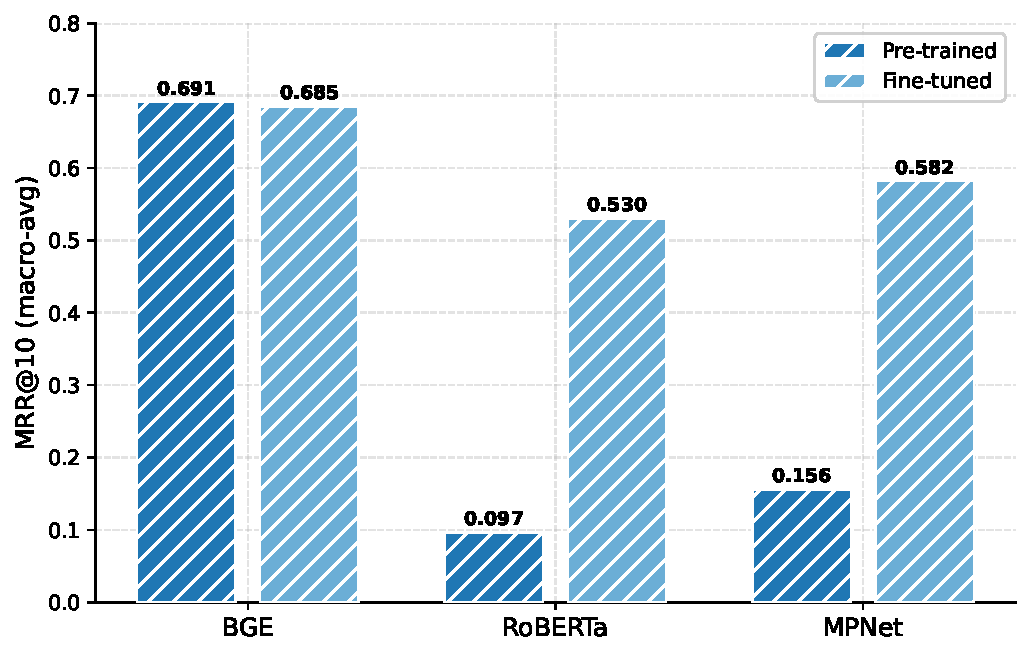
\includegraphics[width=0.75\textwidth]{Figures/fig_float32_baselines.pdf}
%  \caption{Mean MRR@10 (macro-averaged over 13 NanoBEIR subsets) for
%           pre-trained and fine-tuned float32 embeddings across all three
%           backbones.  The large gain for RoBERTa and MPNet and the small
%           decline for BGE are discussed in the text.}
%  \label{fig:float32_baselines}
%\end{figure}

Fine-tuning scores for RoBERTa and MPNet improve a lot from 0.097 to
0.530 and 0.156 to 0.582, respectively. But for BGE, the score almost
doesn't change due to this fine-tuning. In fact, there is a drop of
0.6 pp, which is not statistically significant (paired Wilcoxon
signed-rank test on per-query MRR@10, $p = 0.49$;
Appendix~\ref{sec:significance_bge_finetune}). Because BGE had been
pre-trained for retrieval at a large scale, fine-tuning on a small
corpus would do nothing impactful.

BGE is still ahead of MPNet and RoBERTa by 6.6 and 15.5 percentage
points, respectively. Whether compression methods keep this ranking
across backbones is examined in Section~\ref{sec:cross_backbone}.

%----------------------------------------------------------------------------------------
\section{Post-Hoc Compression}
\label{sec:posthoc_compression}

Here, we look at four methods: INT8 scalar quantisation
(Section~\ref{subsec:int8}), post-hoc binary quantisation
(Section~\ref{subsec:binary}), Product Quantisation
(Section~\ref{subsec:pq}), and TurboQuant (Section~\ref{subsec:tq}).
In Section~\ref{subsec:cross_method}, all these methods are compared
at $32\times$ compression.

%-------------------------------------------
\subsection{INT8 Scalar Quantisation}
\label{subsec:int8}

At $4\times$ compression, the retrieval performance is nearly lossless,
as shown in Table~\ref{tab:int8}. MPNet has the biggest drop from
float32, which is $-1.5$ percentage points (pp).

\begin{table}[H]
  \centering
  \caption[Float32 vs INT8 ($4\times$ compression).]{Mean MRR@10 (macro-averaged over 13 NanoBEIR subsets) for float32 and INT8 ($4\times$ compression). $\Delta$ is the absolute change due to INT8 quantisation.}
  \label{tab:int8}
  \begin{tabular}{| l | c | c | c |}
    \hline
    \textbf{Configuration} & \textbf{BGE} & \textbf{RoBERTa} & \textbf{MPNet} \\ [0.5ex] \hline
    Float32 (fine-tuned)   & 0.685 & 0.530 & 0.582 \\ \hline
    INT8 ($4\times$)       & 0.678 & 0.532 & 0.567 \\ \hline
    \textbf{$\Delta$}      & $\mathbf{-}$\textbf{0.007} & $\mathbf{+}$\textbf{0.002} & $\mathbf{-}$\textbf{0.015} \\ \hline
  \end{tabular}
\end{table}

%-------------------------------------------
\subsection{Binary Quantisation}
\label{subsec:binary}

\begin{table}[H]
  \centering
  \caption[Post-hoc binary quantisation ($32\times$) vs float32 baseline.]{Mean MRR@10 for post-hoc binary quantisation (32$\times$) compared with the fine-tuned float32 baseline.}
  \label{tab:binary}
  \begin{tabular}{| l | c | c | c |}
    \hline
    \textbf{Configuration} & \textbf{BGE} & \textbf{RoBERTa} & \textbf{MPNet} \\ [0.5ex] \hline
    Float32 (fine-tuned)   & 0.685 & 0.530 & 0.582 \\ \hline
    Binary (32$\times$)    & 0.646 & 0.501 & 0.534 \\ \hline
    \textbf{$\Delta$}      & $\mathbf{-}$\textbf{0.039} & $\mathbf{-}$\textbf{0.029} & $\mathbf{-}$\textbf{0.048} \\ \hline
  \end{tabular}
\end{table}

%\begin{figure}[h]
%  \centering
%  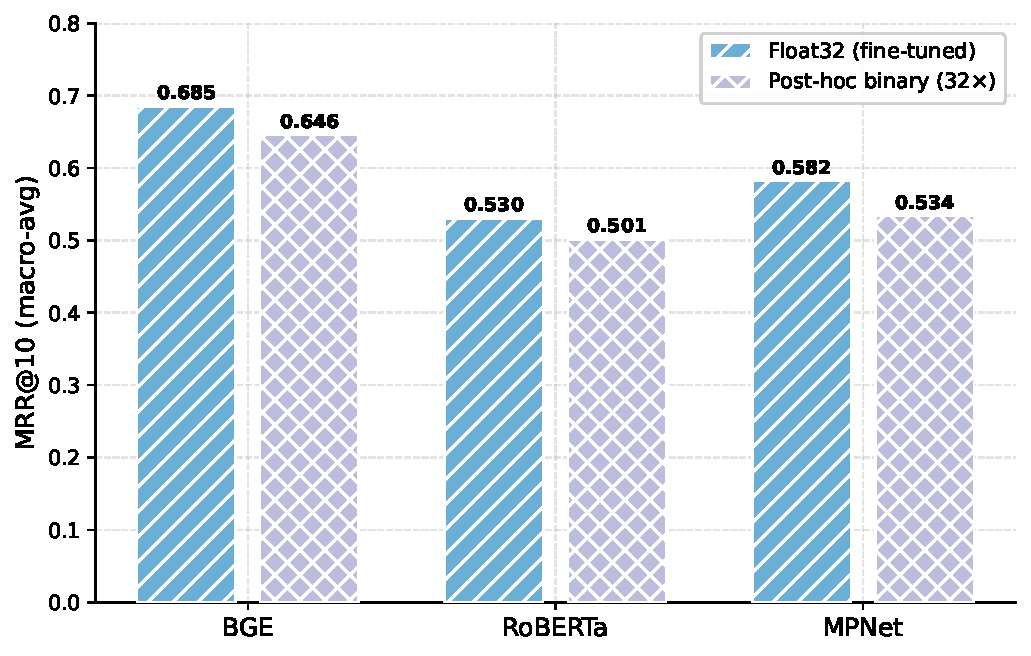
\includegraphics[width=0.75\textwidth]{Figures/fig_binary_quant.pdf}
%  \caption{Mean MRR@10 (macro-averaged over 13 NanoBEIR subsets) for
%           fine-tuned float32 and post-hoc binary embeddings at
%           32$\times$ compression, per backbone.}
%  \label{fig:binary_quant}
%\end{figure}

At $32\times$ compression with post-hoc binary, the quality drops by a
fair amount for all backbones (Table~\ref{tab:binary}): $-4.8$ pp for
MPNet, $-3.9$ pp for BGE, and $-2.9$ pp for RoBERTa. In
Section~\ref{sec:training_compression}, it is shown that training-time
binarisation closes this gap pretty well.

%-------------------------------------------
\subsection{Product Quantisation}
\label{subsec:pq}

We look at thirteen PQ configurations, ranging from $32\times$ to
$384\times$ compression and $n = 4$ and $n = 8$ bits per subspace. The
quality--compression graphs that were made are shown in
Figure~\ref{fig:pq_quality_vs_ratio}.

\begin{figure}[h]
  \centering
  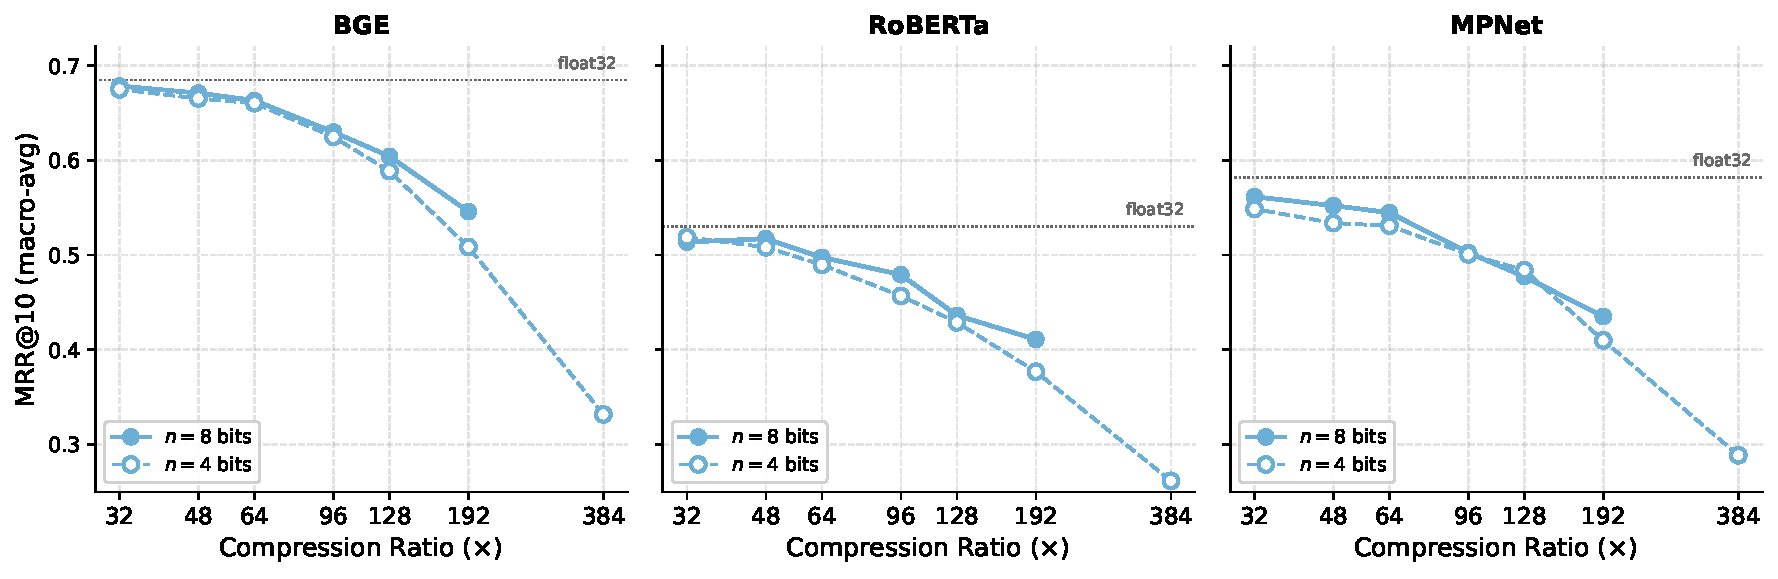
\includegraphics[width=\textwidth]{Figures/fig_pq_quality_vs_ratio.pdf}
  \caption[Product Quantisation: MRR@10 vs compression ratio per backbone.]{Mean MRR@10 (macro-averaged over the 13 NanoBEIR subsets)
           for Product Quantisation as a function of compression ratio,
           one panel per backbone.  Solid lines with filled markers
           use $n = 8$ bits per subspace; dashed lines with hollow
           markers use $n = 4$.  Each point on a curve corresponds to
           a different number of subspaces $M$.  The dotted horizontal
           line marks the fine-tuned float32 baseline for each
           backbone.}
  \label{fig:pq_quality_vs_ratio}
\end{figure}

Two results stand out. First, PQ at $32\times$ is near-lossless, with
quality dropping gracefully until $96\times$ compression, then it drops
significantly. With BGE at $32\times$, when $n = 8$, it scores 0.679,
which is close to the float32 ceiling of 0.685. Second, at any fixed
compression ratio, the $n = 8$ configuration always wins over the
configurations at $n = 4$.

%-------------------------------------------
\subsection{TurboQuant}
\label{subsec:tq}

We test five different TurboQuant (TQ) configurations, ranging from
$4\times$ to $32\times$ compression (8, 4, 3, 2, and 1 bits per
embedding dimension). The quality--compression graphs are shown in
Figure~\ref{fig:tq_quality_vs_ratio}, and the numbers are given in
Table~\ref{tab:tq}.

\begin{figure}[h]
  \centering
  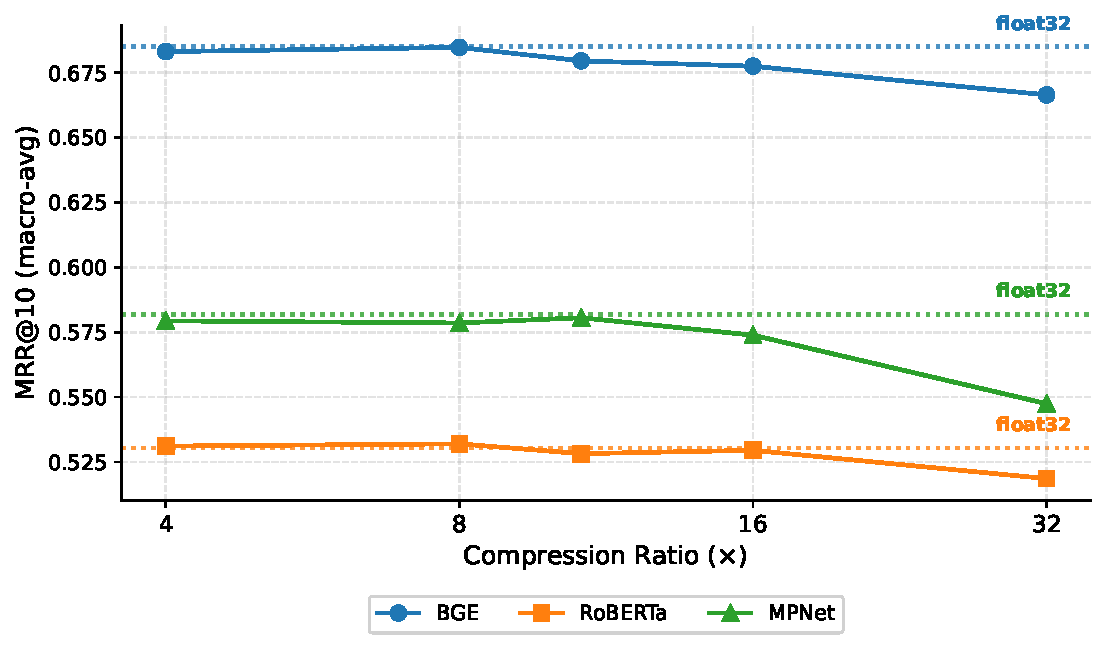
\includegraphics[width=0.85\textwidth]{Figures/fig_tq_quality_vs_ratio.pdf}
  \caption[TurboQuant: MRR@10 vs compression ratio per backbone.]{Mean MRR@10 (macro-averaged over the 13 NanoBEIR subsets)
           for TurboQuant as a function of compression ratio, one line
           per backbone.  Each point corresponds to a bit-width
           $b \in \{1, 2, 3, 4, 8\}$.  The dotted horizontal lines
           mark the fine-tuned float32 baseline for each backbone.}
  \label{fig:tq_quality_vs_ratio}
\end{figure}

\begin{table}[H]
  \centering
  \caption[TurboQuant across five bit-widths vs float32 baseline.]{Mean MRR@10 (macro-averaged over 13 NanoBEIR subsets) for TurboQuant across the five evaluated bit-widths, with the fine-tuned float32 baseline for reference.}
  \label{tab:tq}
  \begin{tabular}{| l | c | c | c | c |}
    \hline
    \textbf{Configuration} & \textbf{Ratio} & \textbf{BGE} & \textbf{RoBERTa} & \textbf{MPNet} \\ [0.5ex] \hline
    Float32 (fine-tuned)   & $1\times$      & 0.685        & 0.530            & 0.582          \\ \hline
    TQ-8bit                & $4\times$      & 0.683        & 0.531            & 0.579          \\ \hline
    TQ-4bit                & $8\times$      & 0.685        & 0.532            & 0.579          \\ \hline
    TQ-3bit                & $10.7\times$   & 0.680        & 0.528            & 0.581          \\ \hline
    TQ-2bit                & $16\times$     & 0.677        & 0.529            & 0.574          \\ \hline
    TQ-1bit                & $32\times$     & 0.666        & 0.519            & 0.547          \\ \hline
  \end{tabular}
\end{table}

TQ-4bit at $8\times$ is almost lossless on all backbones: BGE matches
its float32 ceiling (0.685 vs.\ 0.685), and the curve stays the same
between 4 and 8 bits, making 4 bits per dimension the best working
point. When going from float32 to $32\times$ (1-bit), the loss is
small: BGE loses 1.9 pp, RoBERTa loses 1.1 pp, and MPNet loses 3.5 pp.

%-------------------------------------------
\subsection{Cross-Method Comparison at 32$\times$}
\label{subsec:cross_method}

\begin{figure}[H]
  \centering
  
\includegraphics[width=0.85\textwidth]{Figures/fig_crossmethod_32x.pdf}
  \caption[Cross-method comparison of post-hoc methods at $32\times$.]{Mean MRR@10 (macro-averaged over 13 NanoBEIR subsets) for
           the fine-tuned float32 baseline and the four post-hoc methods
           at $32\times$ compression, grouped by backbone.  Y-axis starts
           at 0.48 to highlight inter-method differences.}
  \label{fig:cross_method_32x}
\end{figure}

\begin{table}[H]
  \centering
  \caption[Four post-hoc methods at $32\times$ vs float32 baseline.]{Mean MRR@10 (macro-averaged over 13 NanoBEIR subsets) for the four post-hoc methods at $32\times$ compression, with the fine-tuned float32 baseline for reference. Best per backbone in bold; ties at displayed precision are bolded together.}
  \label{tab:cross_method_32x}
  \begin{tabular}{| l | c | c | c | c |}
    \hline
    \textbf{Method} & \textbf{Ratio} & \textbf{BGE} & \textbf{RoBERTa} & \textbf{MPNet} \\ [0.5ex] \hline
    Float32 (fine-tuned)                   & $1\times$  & 0.685          & 0.530          & 0.582          \\ \hline
    Post-hoc binary                        & $32\times$ & 0.646          & 0.501          & 0.534          \\ \hline
    TurboQuant, 1-bit                      & $32\times$ & 0.666          & \textbf{0.519} & 0.547          \\ \hline
    PQ, 192 subspaces $\times$ 4-bit codes & $32\times$ & 0.675          & \textbf{0.519} & 0.549          \\ \hline
    PQ, 96 subspaces $\times$ 8-bit codes  & $32\times$ & \textbf{0.679} & 0.514          & \textbf{0.562} \\ \hline
  \end{tabular}
\end{table}

The average MRR@10 for the four post-hoc methods at $32\times$
compression is shown in Table~\ref{tab:cross_method_32x}. The
fine-tuned float32 baseline is used as a comparison. Best per backbone
is shown in bold, and ties at displayed precision are shown in bold
together.

At $32\times$ compression, the best method is dependent on the backbone
(Figure~\ref{fig:cross_method_32x}, Table~\ref{tab:cross_method_32x}).
For BGE and MPNet, PQ ($M{=}96, n{=}8$) wins. But for RoBERTa,
TurboQuant at 1-bit and PQ ($M{=}192, n{=}4$) tie for the winner.
Post-hoc binary has the lowest score across the three backbones.

%----------------------------------------------------------------------------------------
\section{Training-Time Compression}
\label{sec:training_compression}

We look at two groups: binarisation-aware training
(Section~\ref{subsec:ste_atanh}), which aims for the same $32\times$
compression ratio as post-hoc binary quantisation; and Matryoshka
Representation Learning (Section~\ref{subsec:mrl}), which reduces the
number of dimensions.

%-------------------------------------------
\subsection{Binarisation-Aware Training: STE and Annealed Tanh}
\label{subsec:ste_atanh}

We look at two types of binarisation-aware training (BAT) that are only
different in the gradient surrogate used for $\mathrm{sign}(x)$
(Section~\ref{sec:training_time}): BAT-STE (Straight-Through Estimator)
and BAT-atanh (annealed tanh at $\gamma = 0.1$, the principled default
following \cite{yamada2021efficient}; the full ablation over $\gamma \in
\{0.05, 0.1, 0.2\}$ is in Appendix~\ref{sec:gamma_ablation}). At
inference, both make 768-dimensional binary embeddings.

\begin{table}[H]
  \centering
  \caption[Binarisation-aware training vs post-hoc binary at $32\times$.]{Mean MRR@10 at $32\times$ compression for binarisation-aware training methods, post-hoc binary, and the fine-tuned float32 baseline (ceiling). Results are macro-averaged across the 13 NanoBEIR subsets. Best $32\times$ result per backbone in bold. The annealed-tanh annealing rate is fixed at $\gamma=0.1$ throughout; the full ablation over $\gamma$ is reported in Appendix~\ref{sec:gamma_ablation}.}
  \label{tab:ste_atanh}
  \begin{tabular}{| l | c | c | c | c |}
    \hline
    \textbf{Method} & \textbf{Ratio} & \textbf{BGE} & \textbf{RoBERTa} & \textbf{MPNet} \\ [0.5ex] \hline
    Float32 (fine-tuned, ceiling) & $1\times$  & 0.685          & 0.530          & 0.582          \\ \hline
    Post-hoc binary               & $32\times$ & 0.645          & 0.501          & 0.534          \\ \hline
    BAT-STE                       & $32\times$ & \textbf{0.658} & 0.565          & \textbf{0.582} \\ \hline
    BAT-atanh ($\gamma=0.1$)      & $32\times$ & 0.638          & \textbf{0.590} & 0.580          \\ \hline
  \end{tabular}
\end{table}

\begin{figure}[H]
  \centering
  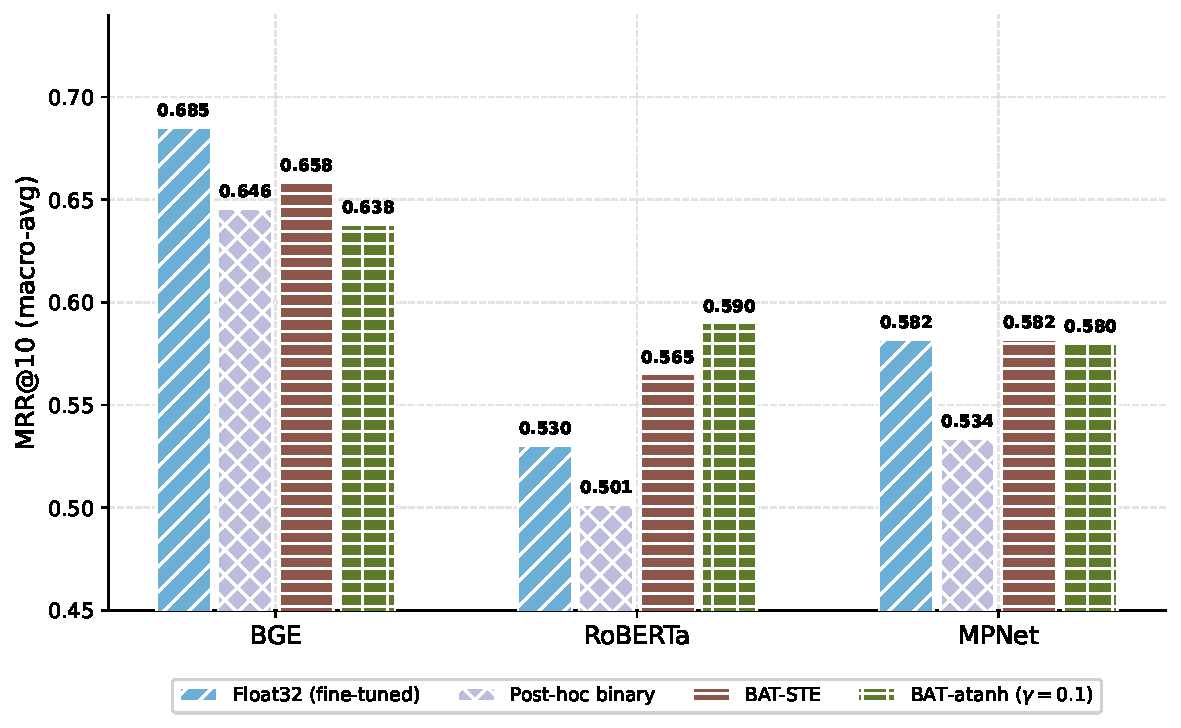
\includegraphics[width=0.85\textwidth]{Figures/fig_bat_atanh_32x.pdf}
  \caption[BAT-STE and BAT-atanh vs post-hoc binary at $32\times$.]{Mean MRR@10 at $32\times$ compression for the fine-tuned
           float32 baseline, post-hoc binary, BAT-STE, and BAT-atanh
           ($\gamma{=}0.1$) across the three backbones. The full
           ablation over $\gamma$ is reported in
           Appendix~\ref{sec:gamma_ablation}.}
  \label{fig:ste_atanh}
\end{figure}

Both versions of BAT are much better than post-hoc binary for all
backbones (Table~\ref{tab:ste_atanh}, Figure~\ref{fig:ste_atanh}). If
you compare BAT-STE to post-hoc binary on BGE, RoBERTa, and MPNet, it
gains 1.3, 6.4, and 4.8 percentage points (pp), respectively. It gets
the biggest gains on the general-purpose backbones whose float32 scores
aren't the best for retrieval. This indicates that when the starting
point isn't already specialised for retrieval, the binarisation
constraint can make the fine-tuning work better. For example, BAT-STE
and fine-tuned float32 have the same performance on MPNet (0.582) and
beat it by 3.5 points on RoBERTa (0.565 vs 0.530; paired Wilcoxon
signed-rank test on per-query MRR@10, $p = 0.005$;
Appendix~\ref{sec:significance_bat_roberta}).

In some backbones, BAT-atanh is better than BAT-STE but doesn't
dominate. BAT-atanh beats BAT-STE on RoBERTa (0.590 vs 0.565, $+2.5$
pp), which is the best performance for RoBERTa, even beating the
float32 fine-tune (0.590 vs 0.530; paired Wilcoxon $p < 10^{-3}$;
Appendix~\ref{sec:significance_bat_roberta}). BAT-STE wins on BGE
($+2.0$ pp) and ties on MPNet ($+0.2$ pp). The ablation in
Appendix~\ref{sec:gamma_ablation} shows the best $\gamma$ differs by
backbone, but no backbone moves by more than 0.014 MRR@10 across
$\gamma \in \{0.05, 0.1, 0.2\}$, so the choice has little practical
effect.

The result that the binarisation-aware variants beat the uncompressed
float32 fine-tune on RoBERTa is surprising, since binarisation removes
information rather than adding it. We analyse this result in three aspects: 
what kind of error it fixes, what geometric property
explains it, and whether it is because of under-training.

\paragraph{The gain is in ranking, not coverage.}
The improvement was seen with MRR@10, but Recall@10 tells a different story.
MRR@10 for BAT-STE on RoBERTa rises from 0.530 to 0.565, and BAT-atanh raises it to 0.590. Both the gains are significant based on the paired Wilcoxon signed-rank test (STE $p=0.005$, atanh $p<0.001$). The Recall@10 doesn't change much (0.553 to 0.552 for STE and to 0.560 for atanh), and the change is also not significant (STE $p=0.57$, atanh $p=0.27$). Therefore, the two methods retrieve the same set of relevant documents as the uncompressed baseline, but the correct answers are placed higher in ranking. We saw improvement on 11 out of 13 NanoBEIR subsets.  The largest gains are
on Touche2020 ($+0.185$), FEVER ($+0.105$), and DBPedia ($+0.096$),
while the recall changes are minimal.

\paragraph{The mechanism is an effective dimension.}
The reason BAT methods achieve a higher ranking can be explained by the geometry of the embedding space. 

Encoders like RoBERTa have embeddings that occupy a narrow cone rather than spreading across all axes~\cite{ethayarajh2019contextual}. We can quantify this with the
\emph{effective dimension} $d_{\text{eff}}$, also called the
participation ratio~\cite{litwinkumar2017optimal, gao2017theory},
\begin{equation}
  d_{\text{eff}} = \frac{\left(\sum_i \lambda_i\right)^2}{\sum_i \lambda_i^2},
\end{equation}
where $\lambda_i$ are the 768 eigenvalues of the centred embedding
covariance matrix. $d_{\text{eff}}$ counts how many dimensions actually
carry variance. This value is 1 if one axis explains all the variance, 768 if the variance is spread evenly.  Table~\ref{tab:effdim} reports
$d_{\text{eff}}$ for the three fine-tuned float32 backbones and the two
RoBERTa BAT variants, computed on the pooled embeddings of the NanoBEIR corpus.

Figure~\ref{fig:roberta_effdim} shows the same models as cumulative
explained-variance curves.

\begin{table}[H]
  \centering
  \caption[Effective dimension across backbones and RoBERTa BAT variants.]{Effective dimension $d_{\text{eff}}$ (participation ratio) of the embedding space, with retrieval quality, on the pooled NanoBEIR corpus. RoBERTa with float32 space has the lowest effective dimension, and binarisation-aware training raises both its effective dimension and its MRR@10.}
  \label{tab:effdim}
  \begin{tabular}{| l | c | c | c | c |}
    \hline
    \textbf{Model} & \textbf{$d_{\text{eff}}$} & \textbf{\% of 768} & \textbf{MRR@10} & \textbf{Recall@10} \\ [0.5ex] \hline
    RoBERTa-FT        & 85  & 11.0\% & 0.530          & 0.553 \\ \hline
    BGE-FT            & 135 & 17.6\% & 0.685          & 0.656 \\ \hline
    MPNet-FT          & 102 & 13.3\% & 0.582          & 0.583 \\ \hline
    RoBERTa-BAT-STE   & 197 & 25.7\% & 0.565          & 0.552 \\ \hline
    RoBERTa-BAT-atanh & 230 & 30.0\% & \textbf{0.590} & 0.560 \\ \hline
  \end{tabular}
\end{table}

\begin{figure}[H]
  \centering
  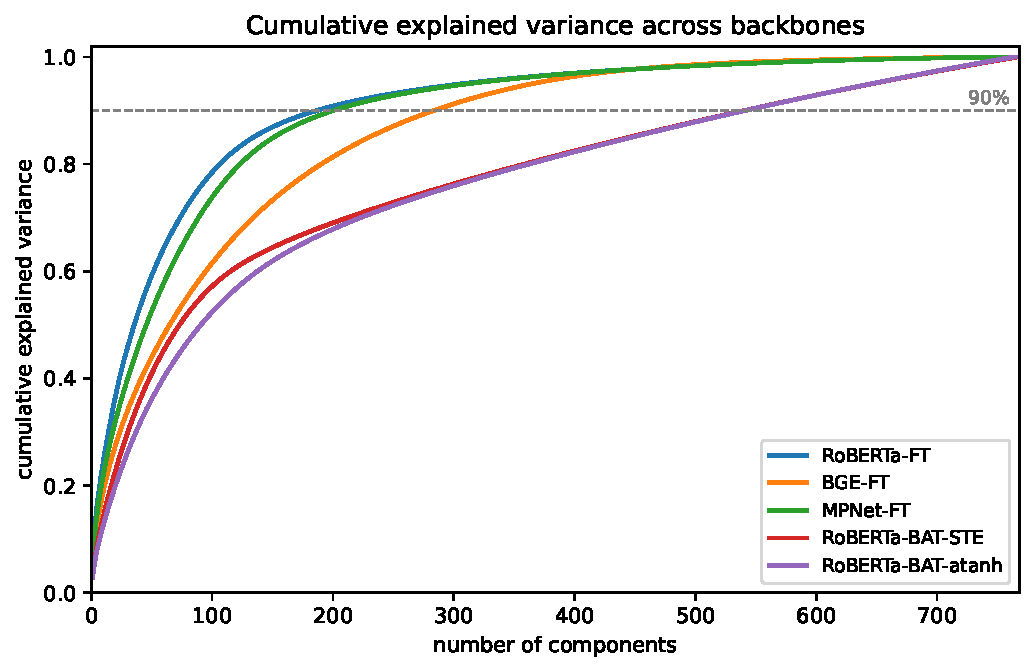
\includegraphics[width=0.85\textwidth]{Figures/fig_roberta_effdim.pdf}
\caption[Cumulative explained variance across backbones.]{Cumulative explained variance against the number of principal
           components, for the three float32 fine-tunes and the two
           RoBERTa BAT variants. A curve that rises quickly indicates a low-effective dimension space. RoBERTa-FT rises
           fastest and RoBERTa-BAT-atanh rises slowest, matching the
           effective-dimension values in Table~\ref{tab:effdim}.}
  \label{fig:roberta_effdim}
\end{figure}

The float32 RoBERTa space is the most compressed of the three backbones
($d_{\text{eff}} = 85$, or $11.0\%$ of 768). Binarisation spreads
variance across more axes and increases the effective dimension of the
binary code to $25.7\%$ for STE and $30.0\%$ for atanh. We observe that MRR@10 and the effective dimension are positively correlated with each other. Similar documents that were previously hard to differentiate can be separated by a space with more useful axes.

\paragraph{This explains why the gain is specific to RoBERTa.}
BGE is pre-trained for retrieval and already has the highest float32
effective dimension ($17.6\%$). It has little anisotropy left to
correct, so binarisation only costs it quality. MPNet sits in between
($13.3\%$) and is close to lossless under BAT. RoBERTa has the most to gain because it begins most compressed. This is the same ordering of
relative benefit, RoBERTa $>$ MPNet $>$ BGE, that the cross-backbone
analysis reports (Section~\ref{sec:cross_backbone}). This clarifies the reason why BAT-atanh is better than BAT-STE on RoBERTa. BAT-atanh generates embeddings that are more spread with the highest $d_{\text{eff}}$, giving the best ranking.

\paragraph{The gain is structural, not under-training.}
A more straightforward reason is that the difference would narrow with additional training because RoBERTa was never trained like BGE on the retrieval task. To test this, we
evaluate an intermediate RoBERTa checkpoint every 2000 steps for the
float32 fine-tune and the two BAT variants
(Figure~\ref{fig:training_trajectory}). But we didn't observe such
convergence. Both BAT variants are clearly above the float32 fine-tune
from the earliest checkpoint, and the gap doesn't change for the rest of
the training. Therefore, rather than being a result of training length, the benefit is a structural feature of the binarized geometry.

\begin{figure}[H]
  \centering
  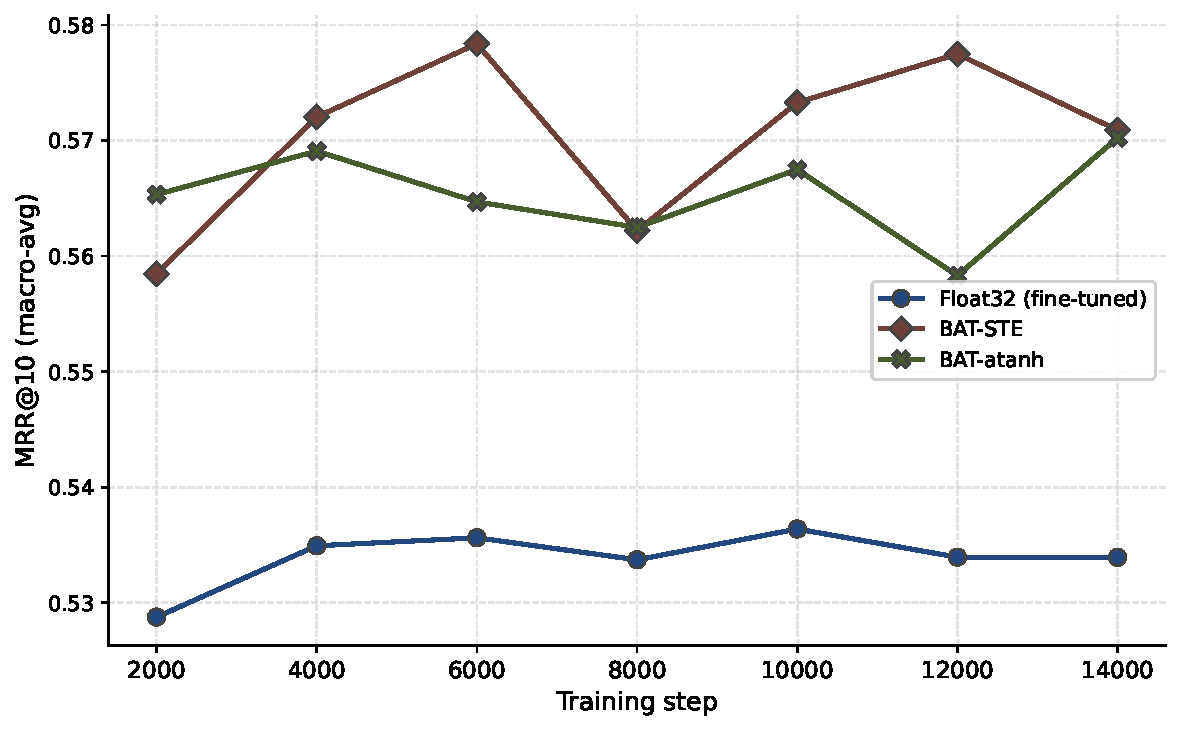
\includegraphics[width=0.85\textwidth]{Figures/fig_training_trajectory.pdf}
  \caption[Training trajectory of binarisation-aware methods on RoBERTa.]{Mean MRR@10 at intermediate RoBERTa checkpoints, evaluated every 2000
           training steps. The gap to
           the float32 fine-tune does not close with more training.}
  \label{fig:training_trajectory}
\end{figure}

%-------------------------------------------
\subsection{Matryoshka Representation Learning}
\label{subsec:mrl}

\begin{figure}[H]
  \centering
  
\includegraphics[width=0.85\textwidth]{Figures/fig_mrl_truncation.pdf}
  \caption[MRR@10 vs MRL truncation dimension across backbones.]{Mean MRR@10 as a function of MRL truncation dimension $d$
           for all three backbones. The right-most point at $d=768$
           is the fine-tuned float32 baseline (no truncation), shown
           with hollow markers.}
  \label{fig:mrl_curve}
\end{figure}

\begin{table}[H]
  \centering
  \caption[MRL truncations across five dimensions vs float32 baseline.]{Mean MRR@10 for MRL truncations across five dimensions, with the 768-dimensional float32 baseline for reference. Compression ratio is $768/d$.}
  \label{tab:mrl}
  \begin{tabular}{| l | c | c | c | c |}
    \hline
    \textbf{Dim}  & \textbf{Ratio} & \textbf{BGE} & \textbf{RoBERTa} & \textbf{MPNet} \\ [0.5ex] \hline
    768 (float32) & $1\times$      & 0.685        & 0.530            & 0.582          \\ \hline
    512           & $1.5\times$    & 0.687        & 0.533            & 0.579          \\ \hline
    256           & $3\times$      & 0.675        & 0.526            & 0.576          \\ \hline
    128           & $6\times$      & 0.639        & 0.513            & 0.560          \\ \hline
    64            & $12\times$     & 0.589        & 0.478            & 0.503          \\ \hline
    32            & $24\times$     & 0.479        & 0.414            & 0.410          \\ \hline
  \end{tabular}
\end{table}

Figure~\ref{fig:mrl_curve} and Table~\ref{tab:mrl} show the retrieval
quality drop as $d$ decreases. At $d = 512$, all backbone models match
their float32 baseline within 0.3 pp. At $d = 256$, all backbones have
losses less than 1 pp. At $d = 128$, the score starts to drop faster.
At $d = 32$, we can see a significant drop in performance from all
backbones (BGE loses 20.6 pp, MPNet 17.2 pp, and RoBERTa 11.6 pp).
Another value of MRL is that it can work with precision-reduction
methods; the stacked combinations are evaluated in
Section~\ref{sec:cross_axis}.

%----------------------------------------------------------------------------------------
\section{Stacked Combinations}
\label{sec:cross_axis}

MRL truncation is paired with a second compression technique in
stacked combinations. We evaluate two taxonomic groups:
pure-training-time stacks (MRL+BAT-STE, MRL+BAT-atanh) and hybrid
stacks (MRL+post-binary, MRL+TQ, MRL+PQ).

Figure~\ref{fig:stacked_combinations} shows the best quality
configuration of each method at various compression ratios across
the three backbones.

\begin{figure}[H]
  \centering
  
\includegraphics[width=\textwidth]{Figures/fig_stacked_combinations.pdf}
  \caption[Stacked compression combinations: MRR@10 vs compression ratio.]{Mean MRR@10 vs compression ratio for the five stacked
           combinations and MRL-only (grey dashed reference) across
           the three backbones. Hollow markers represent
           pure-training-time stacks; filled markers represent
           hybrid stacks. The fine-tuned float32 baseline is shown
           as a horizontal dotted line.}
  \label{fig:stacked_combinations}
\end{figure}

Figure~\ref{fig:stacked_combinations} shows four conclusions.

\paragraph{MRL+PQ dominates the high-compression region.}
At compression ratios $\geq 96\times$, MRL+PQ does best among all
the stacked methods for all backbones. The margin over the
second-best increases as the compression increases. At
192$\times$, MRL+PQ leads by 6.9 pp on BGE, 3.1 pp on RoBERTa, and
4.6 pp on MPNet. At 384$\times$, those gaps grow to 13.0, 6.2, and
7.5 pp.

\paragraph{MRL+BAT-atanh exceeds the float32 baseline for RoBERTa.}
At 32$\times$, MRL+BAT-atanh reaches 0.560, which is 3 pp higher
than the float32 baseline. The only backbone in this method that
allows any configuration to cross its own float32 ceiling is
RoBERTa.

\paragraph{MRL+BAT-atanh beats MRL+BAT-STE.}
Unlike how BAT-atanh beats BAT-STE only for RoBERTa
(Section~\ref{subsec:ste_atanh}), MRL+BAT-atanh dominates
MRL+BAT-STE for all backbones by 1 to 6 pp in the compression
range between 32$\times$ to 384$\times$ (at 96$\times$: BGE
$+$2.9, RoBERTa $+$2.4, MPNet $+$5.1 pp).

The binarisation layer is applied before the MRL loss. STE
converts the floating-point values straight to binary, removing
critical floating-point information required for training, but
tanh still keeps some floating-point information. That could be
the reason MRL+BAT-atanh beats MRL+BAT-STE by some margin for all
backbones across all compression ranges we tried.

\paragraph{Stacking pushes the quality and compression frontier outward.}
The MRL-only line (grey dashed) in
Figure~\ref{fig:stacked_combinations} only goes up to 24$\times$
compression. All stacked curves can go beyond this compression. At
high compression (96$\times$ and above), MRL+PQ dominates the
performance beyond what MRL alone or PQ alone
(Section~\ref{subsec:pq}) can reach. When the two axes of
compression are combined, we can achieve new frontiers of quality
at higher compression ratios. Section~\ref{sec:pareto} follows up
on these findings with Pareto curves.

%----------------------------------------------------------------------------------------
\section{Pareto Frontiers}
\label{sec:pareto}
\label{subsec:pareto_frontiers}

If no other configuration outperforms it in terms of both retrieval
quality and compression ratio, then that configuration is called
\emph{Pareto-optimal}. The collection of such configurations is called
the \emph{Pareto frontier}. Hence, any configuration that is not
included in the Pareto frontier is always worse than some point in it
and should not be selected. The frontier for each backbone is presented
in this section.

\begin{figure}[h]
  \centering
  
\includegraphics[width=\textwidth]{Figures/fig_pareto.pdf}
  \caption[Quality vs compression Pareto frontiers for BGE, RoBERTa, and MPNet.]{Quality vs compression Pareto frontiers for BGE, RoBERTa,
           and MPNet. The $x$-axis is on a log scale. Filled markers
           are Pareto-optimal; hollow markers are dominated. Colour
           encodes method family: post-hoc (blue) vs training-time
           binarisation (orange); float32 baselines are black.}
  \label{fig:pareto}
\end{figure}

\paragraph{BGE frontier.}
Four orders of magnitude of compression are covered by the BGE frontier
(Figure~\ref{fig:pareto}, Table~\ref{tab:pareto_bge}). The Pareto-optimal
configurations from $1\times$ to $96\times$ are listed in
Table~\ref{tab:pareto_bge}; Figure~\ref{fig:pareto} shows that the
frontier extends through stacked MRL+PQ configurations to $1536\times$
(MRR@10 = 0.200).

\begin{table}[H]
  \centering
  \caption[BGE Pareto-optimal configurations.]{BGE Pareto-optimal configurations, ordered by compression ratio. Method family is indicated for each point.}
  \label{tab:pareto_bge}
  \begin{tabular}{| l | c | c | c | c |}
    \hline
    \textbf{Method}                & \textbf{Family} & \textbf{Compression Ratio} & \textbf{Bytes} & \textbf{MRR@10} \\ [0.5ex] \hline
    Pre-trained BGE                & Baseline        & $1\times$                  & 3072           & 0.691           \\ \hline
    MRL-512                        & Post-hoc        & $1.5\times$                & 2048           & 0.687           \\ \hline
    TQ-4bit                        & Post-hoc        & $8\times$                  &  384           & 0.685           \\ \hline
    TQ-3bit                        & Post-hoc        & $10.7\times$               &  288           & 0.680           \\ \hline
    PQ ($M{=}96, n{=}8$)           & Post-hoc        & $32\times$                 &   96           & 0.679           \\ \hline
    MRL-256 + PQ ($M{=}64, n{=}8$) & Post-hoc        & $48\times$                 &   64           & 0.673           \\ \hline
    PQ ($M{=}48, n{=}8$)           & Post-hoc        & $64\times$                 &   48           & 0.663           \\ \hline
    MRL-256 + PQ ($M{=}32, n{=}8$) & Post-hoc        & $96\times$                 &   32           & 0.637           \\ \hline
  \end{tabular}
\end{table}

Three distinct findings emerge from this frontier. At $1\times$, we
have pre-trained BGE and not the fine-tuned one, for the reasons
discussed in Section~\ref{sec:float32_baselines}. TurboQuant dominates
in the moderate range ($8\times$ to $10.7\times$). After $32\times$, PQ
dominates the frontier.

\paragraph{RoBERTa and MPNet frontiers.}
One significant distinction of RoBERTa and MPNet from BGE is that their
$32\times$ frontier point is a training-time binarisation technique
rather than PQ.

\begin{itemize}
  \item RoBERTa at $32\times$: BAT-atanh ($\gamma{=}0.1$) scores 0.590,
        7.1 points higher than the best post-hoc approach
        (PQ ($M{=}192, n{=}4$): 0.519).
  \item MPNet at $32\times$: BAT-STE scores 0.582, which is 2.0 points
        higher than the best post-hoc technique
        (PQ ($M{=}96, n{=}8$): 0.562).
\end{itemize}

For RoBERTa and MPNet, BAT-STE and BAT-atanh are hence clearly
Pareto-optimal at $32\times$.

%----------------------------------------------------------------------------------------
\section{Cross-Backbone Generalisability}
\label{sec:cross_backbone}

Figure~\ref{fig:cross_backbone} presents \emph{quality retention}
(compressed MRR@10 divided by the same backbone's float32 MRR@10)
rather than raw MRR@10.

All three backbones have some starting-point retrieval capability after
fine-tuning (Section~\ref{sec:float32_baselines}). To eliminate this
absolute quality gap, we normalise by each backbone's own float32 ceiling.

\begin{figure}[h]
  \centering
  
\includegraphics[width=0.95\textwidth]{Figures/fig_cross_backbone.pdf}
  \caption[Quality retention and cross-backbone std across configurations.]{Quality retention (compressed MRR@10 divided by the same
           backbone's float32 MRR@10) for a representative set of
           configurations, arranged by compression ratio. The standard
           deviation of retention for each of the three backbones is
           displayed in the rightmost column.}
  \label{fig:cross_backbone}
\end{figure}

BAT-STE (std $0.043$) and BAT-atanh (std $0.075$) have the highest
variance across backbones. The relative gain from these approaches is
in the order: RoBERTa $>$ MPNet $>$ BGE, as shown in
Section~\ref{subsec:ste_atanh}. The remaining configurations are mostly
stable and are backbone-invariant.

